\subsection{Brechungsindex und Dispersion}
    In einem elektromagnetischem Wechselfeld wird bei hoher Frequenz (bspw. sichtbares Licht) der Brechnungsindex
    $$
    n = \sqrt{ \varepsilon \mu}\quad\text{(bei Permeabilität } \mu = 1: \quad n = \sqrt{ \varepsilon }) 
    $$
    in Abhängigkeit von der dielektrischen Konstante $\epsilon$ gemessen.
    $\mu$ und $\varepsilon$ sind frequenzabhängig, da die Beiträge zur Polarisation, Verschiebung und Orientierung ebenfalls von der Frequenz abhängen.

    \begin{definition}{Dispersion}
        Dispersion bedeutet, dass die dielektrische Konstante $\epsilon$ und der Brechungsindex $n$ von der Frequenz der anregenden elektromagnetischen Wellen abhängen.
    \end{definition}
    
    \begin{minipage}{0.45\linewidth}
        \paragraph{Lorentz-Modell} Zur Beschreibung der Dispersion werden die Moleküle als gedämpfte harmonische Oszillatoren genähert. Dazu wird die Analogie zu einem Federpendel gemäß \autoref{fig:I.2_federpendel} betrachtet.\\
    \end{minipage}\hspace{0.5cm}
    \begin{minipage}{0.5\linewidth}main.pdf
        \centering
        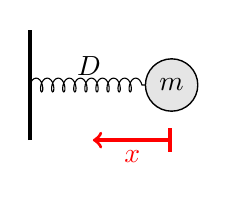
\begin{tikzpicture}
            \draw[decorate,decoration={coil,segment length=4pt}] (0,0)   --node[midway, above]{$D$} (1.5,0);
            \node[draw, circle, minimum size=0.6cm, line width=0.5pt, fill=black!10] at (1.8,0) {$m$};
            \draw[ultra thick] (0,-0.7) -- (0,0.7);
            %\draw (0,-0.7) -- (2.5,-0.7);
            \draw[|->, red, very thick] (1.8, -0.7) --node[midway, below]{$x$} (0.8, -0.7);
        \end{tikzpicture}
        \captionof{figure}{Harmonischer Oszillator einer Masse $m$ mit Federkonstante $D$, Dämpfungskonstante $\gamma$ und Auslenkung $x$.}
        \label{fig:I.2_federpendel}
    \end{minipage}

	Durch das Licht besteht das E-Feld
	$$
	E = E_0 e^{i \omega t}.
	$$
	Die Differentialgleichung des getriebenen, gedämpften Oszillators ist
	\begin{equation}
		\label{2.19}
		m \ddot{x} + \gamma \dot{x} + m \omega_0^2 = \mathrm{e} E_0 e^{i \omega t}
	\end{equation}
	mit der stationären Lösung 
	$$
	x\left( t \right) = X e^{i \omega t},
	$$
	wobei
	\begin{align}
		{X} &= \frac{ \mathrm{e} E_0}{ m \left( \omega_0^2-  \omega^2 \right) + i \gamma \omega}\\
		\label{eq:2.21}
		&= \left[ \frac{\mathrm{e} m\left( \omega_0^2 - \omega^2 \right) }{ m^2 \left( \omega_0^2 - \omega^2 \right) + \left( \gamma \omega \right) ^2} -i \frac{\mathrm{e} \gamma }{m^2\left( \omega_0^2 - \omega^2 \right) + \left( \gamma \omega \right) ^2} \right].
	\end{align}
	Die Schwingung erzeugt ein Dipolmoment $p = \mathrm{e}x$. Die Dielektrizitätskonstante $ \varepsilon\left( \omega \right) $ lautet mit Gleichung \eqref{2.8} und \eqref{eq:2.11}
	\begin{equation}
		\label{eq:2.22}
		\varepsilon = 1 + \frac{N}{ \varepsilon_0} \alpha = 1 + \frac{N}{ \varepsilon_0} \frac{\mathrm{e}x}{E_0}.
	\end{equation}
	Daraus folgt mit der komplexen Lösung der DGL \eqref{eq:2.21}
	\begin{equation}
		\varepsilon = \varepsilon' - i \varepsilon''.
	\end{equation}
	Für den komplexen Brechungsindex $\tilde n$ gilt mit $\mu=1$
	\begin{equation}
		\Tilde{n} = \sqrt{ \varepsilon \mu}  = \sqrt{ \varepsilon} = \sqrt{ \varepsilon' - i \varepsilon''} =: n + i \kappa,
	\end{equation}
	wobei $n$ die Dispersion und $ \kappa$ die Absobtion beschreiben. Die Frequenzabhängigkeit dieser beiden Komponenten $n$ und $\kappa$ ist in \autoref{fig:vl03_kramers_kronig} dargestellt.\\
	\begin{figure}[H]
	\centering
		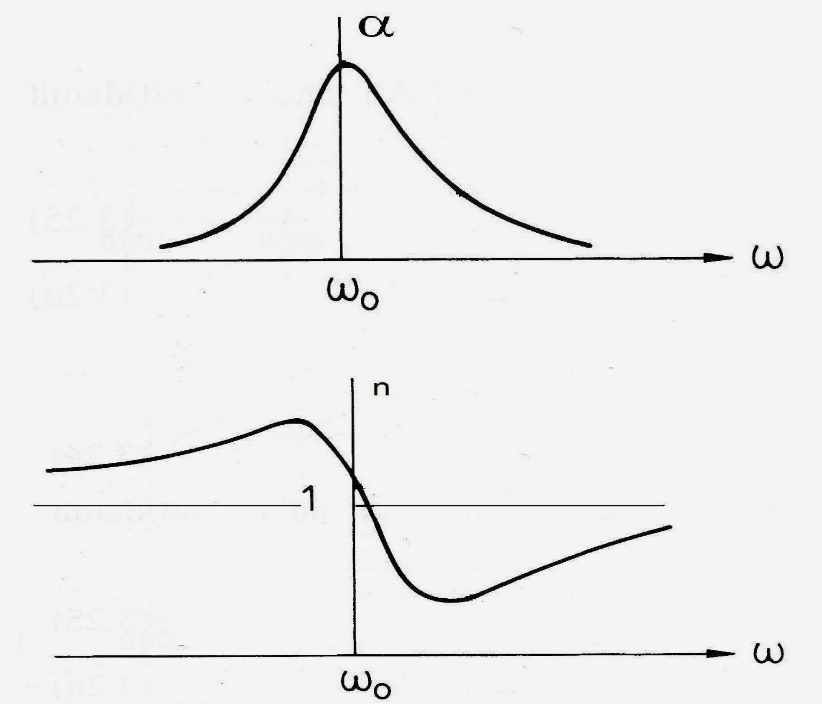
\includegraphics[width=7cm]{figures/vl03/vl03_brechungsindex_kramers_kronig.png}
		\caption{Refaktion $n$ und Absorbtion $\alpha$, bzw. $\kappa$, sind abhängig von der Frequenz $\omega$ des induzierenden Lichts \cite{Haken_Wolf_2006}. Die Beziehung zwischen diesen beiden Größen wird durch die Kramers-Kronig-Beziehung beschrieben.}
		\label{fig:vl03_kramers_kronig}
	\end{figure}

	Dieses Modell kann auf die Quantenmechanik erweitert werden, wobei jedes Molekül als eine Menge an Oszillatoren fungiert. Die Dielektrizitätskonstante ist dann die Summe
	\begin{equation}
		\varepsilon' \left( \omega \right) = 1 + \chi_{\text{el}} + \chi_{\text{ion}} + \chi_{\text{or}}
	\end{equation} 
	der elektrischen Verschiebungpolarisation $ \chi_{\text{el}}$, der ionischen Verschiebungspolarisation $\chi_{\text{ion}}$ und der Orientierungspolarisation $\chi_{\text{or}}$. Deren Frequenzabhängigkeit wird in \autoref{fig:vl03_freq-abh_dielektr-zahl} dargestellt.
	\begin{figure}[H]
		\centering
		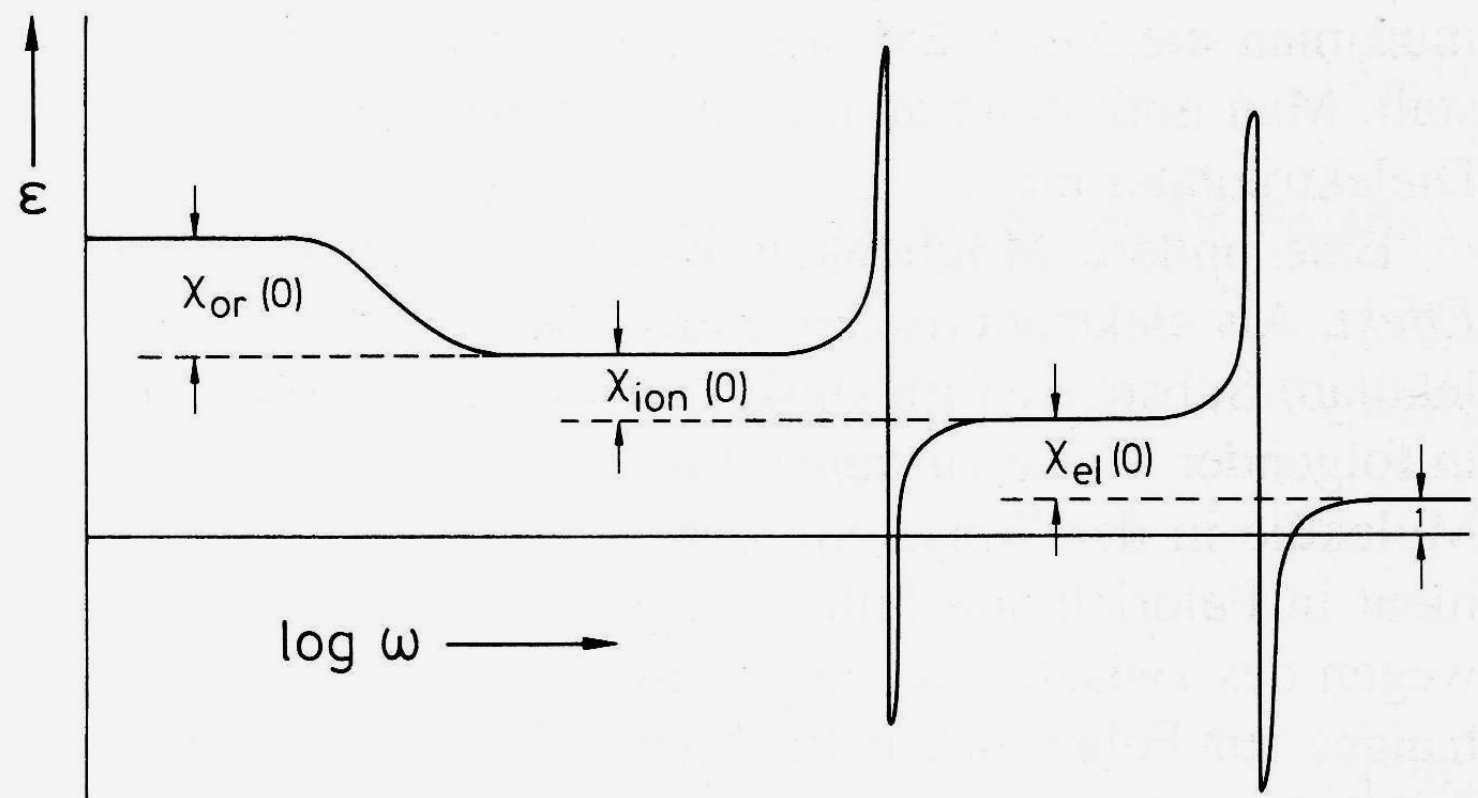
\includegraphics[width=0.7\linewidth]{figures/vl03/vl03_epsilon_frequency_dependency.png}
		\caption{Dielektrizitätskonstante $\epsilon$ in Abhängigkeit der Frequenz $\omega$ der anregenden EM-Wellen. Die Polarisationseffekte $\chi$ treten nur bis zu bestimmten Frequenzen auf. Für sehr hohe Frequenzen vereinfacht sich sogar $\epsilon \to 1$, da die Polarisationseffekt verschwindet klein werden.}
		\label{fig:vl03_freq-abh_dielektr-zahl}
	\end{figure}

\subsection{Moleküle in magnetischen Feldern}
	Die magnetischen Eigenschaften eines Moleküls können aus seinen makroskopischen Größen abgeleitet werden. Wir erinnern uns im Folgenden an einige Definitionen aus der Elektrodynamik. So gilt für die magnetische Feldstärke in einem Medium $ \Vec{B}$
	\begin{equation}
		\label{eq:2.26}	
		\Vec{B} = \mu \Vec{B}_{0}
	\end{equation}
	mit der magnetischen Permeabilität des Mediums $ \mu$ und der magnetischen Feldstärke ohne Medium $ \Vec{B}_{0}$. 
	Die Magnetisierung ergibt sich nach
	\begin{equation}
		\label{eq:2.27}
		\Vec{M} = \frac{1}{ \mu_0} \left( \Vec{B} - \Vec{B}_{0} \right) 
	\end{equation}
	während sich die magnetische Suszeptibilität $ \chi_{m}$ durch
	\begin{equation}
		\chi_{m} = \mu-1
	\end{equation}
	berechnen lässt. Zusätzlich lässt sich die Feldstärke $\vec B$ durch die Flussdichte $\vec H$ mit
	\begin{equation}
		\label{eq:2.29}
		\Vec{B} = \mu \mu_0 \Vec{H}
	\end{equation} 
	und 
	\begin{equation}
		\label{eq:2.30}
		\vec B_0 = \mu\vec H		
	\end{equation}
	ausdrücken. Materialien mit einer magnetischen Suszeptibilität von
	$$
	\chi_{m} <0 \quad \left( \mu <1 \right) 
	$$ 
	sind \quickdef{diamagnetisch}, wohingegen Materialien mit
	$$
	\chi_{m}>0 \quad \left( \mu > 1 \right) 
	$$ 
	\quickdef{paramagnetisch} sind und ein permanentes magnetisches Moment besitzen. Die magnetische Suszeptibilität lässt sich durch verschiedene Methoden bestimmen:
	\begin{itemize}
		\item Elektronen-Spin-Resonanz (ESR)
		\item In einem inhomogenen magnetischen Feld $\vec H$ erfährt eine Probe eine Kraft
			$$
			F \sim \chi_{m} \frac{\partial | \Vec{H} | }{\partial x},	
			$$ 
			woraus die magnetische Suszeptibilität $\chi_m$ gefittet werden kann.
	\end{itemize}

	Ein para- oder diamagnetisches Objekt mit dem Volumen $V$ erfährt in einem Feld $\Vec{H} = \vec B_0/ \mu_0$ die Magnetisierung
	\begin{equation}
		\label{eq:2.31}
		\Vec{M} = \chi_{m} \Vec{H} = \chi_{m} \frac{\vec B_0}{ \mu_0}.
	\end{equation}

	Analog zur Polarisierung $\Vec{P} = N \Vec{p'}$ eines Objekt in einem elektrischen Feldern gilt in einem magnetischen Feld
	\begin{equation}
		\label{2eq:.32}
		\Vec{M} = N \Vec{m}'
	\end{equation}
	mit
	$$
	N = \frac{n}{V} = \frac{\text{Teilchenzahl}}{\text{Probenvolumen}}
	$$ 
	und
	\begin{equation}
		\label{eq:2.33}
		\Vec{m}' = \frac{\Vec{M}}{N} = \frac{ \chi_{m} B_0}{N \mu_0} = \frac{\left( \mu -1 \right) B_0}{N \mu_0}.
	\end{equation}
	Im molekularen Bild entspricht die Magnetisierung $\Vec{M}$ der Summe der zeitlich gemittelten Beiträge $\Vec{m}'$ von $n$ Molekülen. \\[-1em]
	
	Insofern nur Diamagnetismus besteht, also $\Vec{m}' = \vec m_{\text{ind}}$ gilt, können magnetische Momente immernoch durch ein externes magnetisches Feld induziert werden.

	\subsection{Diamagnetische Moleküle} 
	Moleküle besitzen oft kein permanentes magnetisches Moment. So summieren sich bei einer gradzahligen Menge an Elektronen die Drehimpulse zu null:
	$$
	\Vec{L}_{\text{tot}} = 0, \quad \Vec{S}= 0 , \quad \Vec{J} = 0 
	$$
	Trotzdem kann mit Hilfe eines externen Feldes $\Vec{B}_{0}$ ein magnetisches Moment $\Vec{m}_{\text{ind}}$ induziert werden, welches laut Lenz'scher Regel seiner Ursache entgegenwirkt. Es folgt
	\begin{align}
		\label{eq:2.34}
		\Vec{m}_{\text{ind}} &= \beta \Vec{B}_{0}\\
		\Rightarrow  \qquad\beta &< 0,
	\end{align}
	wobei $\beta$ die magnetische Polarisierbarkeit ist. Mit Gleichung \eqref{eq:2.33} und \eqref{eq:2.34} ergibt sich die
	\begin{important}
		Beziehung zwischen mikroskopischer, magnetischer Polarisierbarkeit $\beta$ und makroskopischer magnetischen Suszeptibilität $\chi_m$
		$$
		\beta = \frac{\chi_{m}}{N \mu_0}.
		$$
	\end{important}
	\paragraph{Beispiel 1: Wasserstoff \ce{H2}}  Das diamagnetische Wasserstoff Molekül \ce{H2} hat die magnetische Suszeptibilität
	$$
	\beta = -\SI{2,4}{\cdot 10^{-30} \ampere \meter^4 \per \volt \second}
	$$
	\paragraph{Beispiel 2: Größenordnungen} 
	In einem magnetischen Feld $\Vec{B}_{0} = \SI{1}{\volt \second \per \meter \squared } = \SI{1}{\tesla}$ ist das molekular induzierte magnetische Moment
	$$
	m_{\text{ind}} = \SI{-3}{\cdot 10^{-30} \frac{\ampere \meter^4}{\volt \second} } \cdot \SI{1}{ \frac{\volt \second}{\meter^2} }= \SI{-3 }{\cdot 10^{-30} \ampere \meter^2}.
	$$ 
	Es ist um 6 Größenordnungen kleiner ist als das Bohr'sche Magneton
	$$
	\mu_{\text{B}} = \SI{9,27}{\cdot 10^{-24} \ampere \meter^2} = \frac{\mathrm{e} \hbar }{2 m_0},
	$$
	welches die Einheit des Magnetismus eines Elektrons im ersten Bohrradius mit Drehimpuls $\hbar $ ist.\\
	\paragraph{Beispiel 3: Benzen \ce{C6H6}} 
	Benzen ist stark anisotrop mit
	$$
	\mu_0 \beta_{\perp} = \SI{-152}{\cdot 10^{-36} \meter \cubed} \quad \text{und}\quad \mu_0 \beta_{ \|} = \SI{-62}{\cdot 10^{-36}\meter \cubed}.
	$$
	\autoref{fig:vl03_benzen} erklärt die Bezeichnungen $\parallel$ und $\perp$ und zeigt die Orbitalstruktur von Benzen. $\pi$-Elektronen können leicht in der Ebene des Moleküls auf ein induziertes Magnetfeld reagieren, da sie entlang der konjugierten Doppelbindungen delokalisiert sind - es kommt zu sogenanntem \quickdef{molekularen Wirbelstrom}.\\
	Anmerkung: Die Diamagnetische Suszeptibilität nimmt zu bei größerer Elektronenmobilität entlang geschlossener Schleifen und senkrecht angelegten magnetischen Feldern.
	\begin{figure}[H]
		\centering
		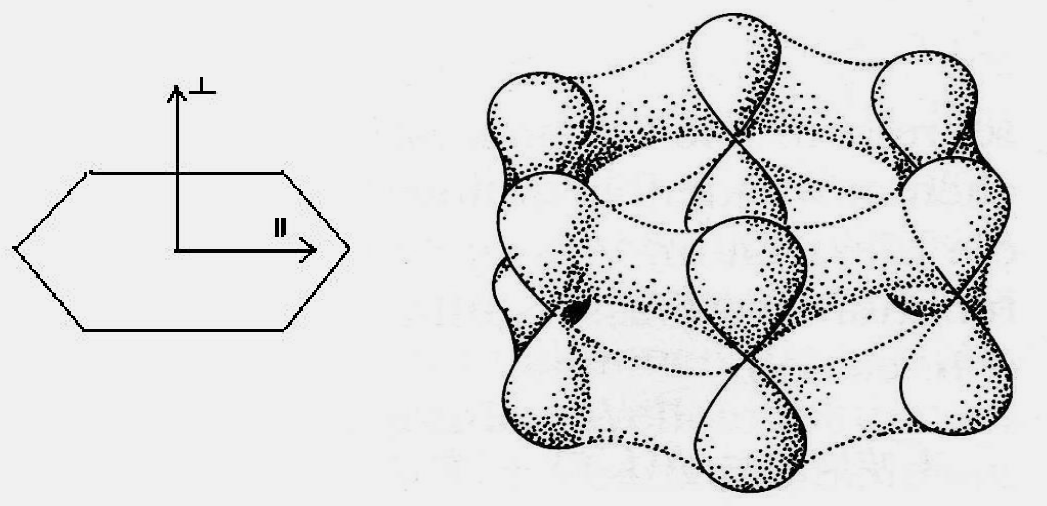
\includegraphics[width=0.9\linewidth]{figures/vl03/vl03_benzen.png}
		\caption{links: Beschriftung der Richtungen $\parallel$ und $\perp$ im Benzen-Molekül.\\
		rechts: $\pi$-Orbitale des Benzen-Moleküls, in welchen sich die Elektronen frei um den Ring bewegen.}
		\label{fig:vl03_benzen}
	\end{figure}


\subsection{Paramagnetische Moleküle}
	\paragraph{Satz von Curie}
	Vorraussetzung für Paramagnetismus in Molekülen ist das Vorhandensein eines permanenten Dipolmoments. Solche Moleküle sind zum Beispiel
	\begin{itemize}
		\item \ce{O2}, \ce{S2} (Gase): Diese Moleküle haben im elektronischen Grundzustand ein Triplett mit Gesamtspin $S=1$.
		\item Radikale, also Moleküle mit ungepaartem elektronischen Spin $S=\frac{1}{2}$.
		\item Organische Moleküle in metastabilen Triplet-Zuständen $S = 1$.
	\end{itemize}
	Sowohl der Spin als auch der Drehimpuls kann zum Paramagnetismus beitragen.\\

	Ähnlich zur Orientierungspolarisation im elektrischen Feld konkuriert die Orientation der magnetischen Dipole 
	$$
	W_{\text{or}} = - \Vec{m}_{p}\cdot\Vec{B}_{0}
	$$ 
	mit der thermischen Bewegung 
	$$
	W_{\text{th}} \sim \mathrm{k}_{\mathrm{B}} T.
	$$
	In verdünnten Systemen findet wegen der Teilchenabstände nahezu keine Interaktion zwischen Molekülen statt. In solchen Systemen gilt {bei hohen Temperaturen}
	\begin{equation}
		\label{eq:2.36}
		m' = \frac{1}{3} \frac{\Vec{m}_{p}\cdot\Vec{B}_{0}}{\mathrm{k}_{\mathrm{B}} T} \Vec{m}_{p}.
	\end{equation}
	\begin{verbal}
		Die Näherung gilt nur für große $T$, da analog zur Orientierungspolarisation eine Näherung der Langevin-Funktion (vgl \autoref{fig:vl2_langevin}) mit einem Argument $\to 0$ gemacht wird.
	\end{verbal}
	Das gemittelte magnetische Dipolmoment $m'$ wird bei hohen Temperaturen also analog zum orientierten elektrischen Dipolmoment $P_\text{or}'$ nach Gleichung \eqref{eq:2.16} beschrieben.
	$m'$ ist der Beitrag einzelner Moleküle mit einem paramagnetischem Moment $m_{p}$ zum makroskopischen magnetischen Moment 
	\begin{equation}
		\label{eq:2.37}
		\Vec{M} = N \frac{1}{3} \frac{m_{p}^2 \Vec{B}_{0}}{\mathrm{k}_{\mathrm{B}}T}.
	\end{equation}
	Daraus folgt der
	\begin{important}
		\textbf{Satz von Curie}\\
		\begin{equation}
			\label{eq:2.38}
			\chi_{m} = N \frac{1}{3} \frac{ \mu_0 m_{p}^2}{\mathrm{k}_{\mathrm{B}} T}
		\end{equation}
		\textbf{bei hohen Temperaturen $T$.}
	\end{important}

	\paragraph{Quantenmechanische Beschreibung}
	Für $ \alpha m \to m_{p}^2$ gilt nach dem Erwartungswert des magnetischen Dipolmoments 
	$$
	\braket{\mu} = g_{j}^2 \mu_{B}^2 j\left( j+1 \right).
	$$ 
	Die gesamte magnetische Suszeptibilität beträgt somit
	$$
	\begin{aligned}
		\mu &= 1 + \chi_\text{dia} + \chi_\text{para} \\
			&= 1 + N\left( \mu_0 \beta_{\text{dia}} + \frac{ \mu_0 m_{p}^2}{3 \mathrm{k}_{\mathrm{B}}T} \right)  = 1+ \chi.
	\end{aligned}
	$$
	Die mikroskopischen Größen $ \beta_{\text{dia}}$ und $m_{p}$ werden bestimmt durch Auftragung der makroskopischen Werte $ \mu$ und $ \chi$ über $ 1 /T$. Die Vorgehensweise ist also analog zur Bestimmung mikroskopischer Größen, welche Verschiebungs- und Orientierungspolarisation im elektrischen Feld beschreiben.


